\documentclass{article}
\usepackage[utf8]{inputenc}
\usepackage{tikz}
\usetikzlibrary{positioning}
\usetikzlibrary{shapes}

\begin{document}

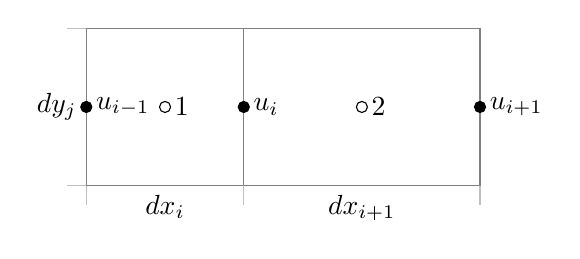
\begin{tikzpicture}
%grid
%horizontal
\draw[gray, thin] (-2,1) -- (3,1);
\draw[gray, thin] (-2,-1) -- (3,-1);
%vertical
\draw[gray, thin] (-2,1) -- (-2,-1);
\draw[gray, thin] (0,1) -- (0,-1);
\draw[gray, thin] (3,1) -- (3,-1);
%anchor lines
\draw[lightgray, thin] (-2,-1) -- (-2,-1.25);
\draw[lightgray, thin] (0,-1) -- (0,-1.25);
\draw[lightgray, thin] (3,-1) -- (3,-1.25);

\draw[lightgray, thin] (-2,-1) -- (-2.25,-1);
\draw[lightgray, thin] (-2,1) -- (-2.25,1);
%nodes
\filldraw [black] (0,0) circle (2pt) node[anchor=west] {$u_{i}$};
\filldraw [black] (3,0) circle (2pt) node[anchor=west] {$u_{i+1}$};
\filldraw [black] (-2,0) circle (2pt) node[anchor=west] {$u_{i-1}$};
%dx dy anchors
\node[black, thin, anchor=north](dxi) at (-1,-1){$dx_i$};
\node[black, thin, anchor=north](dxip) at (1.5,-1){$dx_{i+1}$};
\node[black, thin, anchor=east](dyjm) at (-2,0){$dy_{j}$};
%center nodes
\draw [black] (1.5,0) circle (2pt) node[anchor=west] {$2$};
\draw [black] (-1,0) circle (2pt) node[anchor=west] {$1$};
\end{tikzpicture}
\end{document}
